\documentclass{ppig}
\usepackage{epsfig, graphicx} % support for image encoding and manipulation
\usepackage{ucs} % support for using UTF-8 as input encoding in LaTeX
\usepackage[utf8x]{inputenc} % required for UTF-8 support with ucs.sty
\usepackage{tabularx, multirow, booktabs} % support for high-quality tables

% The titlebox defines how much vertical space is given for
% the authors' list. If you need extra space to show all the
% authors, uncomment the line below and increase the value. Please
% do not make the titlebox smaller than the original size of 5cm.
%\setlength\titlebox{5cm}

\title{Problem-Solving in Programming: A Metacognitive Examination of IDE Design}

% List the authors like you would in a table.
% The \And command creates another author's column. Use it after the
% details of one author to separate them from the following author horizontally.
% The \AND command creates a new "row" of authors and it should be used
% when the authors don't fit on the same line. You may have to increase
% the titlebox so that the author's don't overlap with the abstract.
\author{Nicholas Nelson \\
  Electrical Engineering \&\\ Computer Science \\
  Oregon State University \\
  nelsonni@oregonstate.edu \\
  \And
  Anita Sarma \\
  Electrical Engineering \&\\ Computer Science \\
  Oregon State University \\
  Anita.Sarma@oregonstate.edu \\
  \And
  André van der Hoek \\
  Department of Informatics \\
  University of California, Irvine \\
  andre@ics.uci.edu
}
  
\date{\today}

% Packages and macros for editorial purposes. Not required for submission.
\usepackage{color}
\definecolor{darkgreen}{rgb}{0.0, 0.5, 0.0}
\definecolor{ballblue}{rgb}{0.13, 0.67, 0.8}
\definecolor{aoblue}{rgb}{0.0, 0.0, 1.0}
\newcommand{\bold}[1]{\textit{\textbf{\color{aoblue}#1}}}
\newcommand\tab[1][1cm]{\hspace*{#1}}
\usepackage{enumitem}

\begin{document}
\maketitle
\thispagestyle{empty}

\begin{abstract}

Software development encompasses more than generating, testing, and maintaining code.
It is fundamentally about harnessing cognitive problem-solving skills to develop solutions to computational problems expressed in code.
Contemporary IDEs natively support the code-centric aspects of software development, but forego providing direct support for many of the metacognitive aspects.
Examples of these metacognitive aspects include constructing models, recalling prior knowledge, interpreting code artifacts, and reflecting on work.
In this paper, we examine support in modern IDE design for three of the metacognitive problem-solving aspects: (1) articulating \& refining alternatives, (2) understanding \& assessing alternatives, and (3) recombining aspects of alternatives.
Based upon our observations, we propose a new user interface for IDEs which enables previously underrepresented aspects of problem-solving; specifically addressing the disparity in support for these three aspects. 
\end{abstract}

\section{Introduction}
\bold{Introduction to programming as problem-solving\\}
Software developers create multiple versions of code to explore and compare viable alternative solutions.
These alternative solutions are not static artifacts that are thrown away during the next garbage collection cycle; they are manipulated, evaluated, broken apart, and recombined into a final version that is optimized for the requirements the developer desires most.
In many cases, the act of writing code is a small part of the larger activity that goes into solving computational problems.
Programming is not merely about language syntax and semantics~\cite{loksa2016programming}.
There are aspects of software development that involve the creation, use, and preservation of artifacts that are devoid of code.
These artifacts have a profound impact on the act of programming, the code that results from programming, and whether a developer is successful in addressing a target problem.

\bold{Scenario to illustrate programming as problem-solving\\}
Imagine a scenario in which Sally, a junior developer, is working on migrating a leaderboard feature from a previously released mobile game.
Her company has decided to release an updated version of the game, and along with new levels and gameplay elements, they have decided to allow users to connect their in-game scores to a shared platform that connects mobile game enthusiasts across different games.
To begin, Sally assigns the task to herself in the issue tracker and examines the requirements and design constraints documented through consumer research conducted by the marketing department.
She explores several different ideas by \textit{sketching out alternative designs}, using each alternative as a chance to think creatively and capture new thoughts as they develop.
After exhausting her initial ideas for solutions, she begins \textit{working through} each design to determine the feasibility of each alternative.
When the infeasible or impractical solutions have been removed, Sally begins to \textit{weigh different strengths and weaknesses of the alternative solutions under consideration}.
This results in several candidate solutions that Sally believes contain aspects best suited for this situation, and she takes these \textit{different aspects and combines them into a new solution}.
This process can involve code exploration, but the primary focus is on enacting a computation solution arising from metacognitive problem-solving activities.

When examining the support for these implicit aspects of problem-solving among developer tools, there is a gap that appears among problem-solving steps that do not directly hinge upon interaction with code.
Modern IDEs focus on the syntactic activities of code generation, examination, maintenance, and execution.
But the cognitive steps that lead into that code-based activity are not as well understood or supported.
Therefore, we take a step back and examine the user interfaces (UI) of modern IDEs to understand which aspects of problem-solving are supported and which can be supported through a reimagined interface.
More specifically, we focus on \textbf{developing strategies} (from the \textit{Activity} column of Table~\ref{matrix}) since this activity, and it's accompanying actions, are not well supported by the UI of modern IDEs.
We are exploring different IDEs based on this new paradigm of programming as problem-solving.
For this exploration, we are working on a cards-based environment.
This environment is our attempt at how we think an alternative environment would function when supporting the entire range of problem-solving activities, irregardless of whether an action directly involves code.
This concept provides the user with flexibility in orienting their workspace according to task-specific needs and composing different configurations that enable comparisons, examinations, and recombinations of alternatives in a side-by-side fashion.

\section{Programming as Problem-Solving}
\bold{Introduction to our model of programming as problem-solving, and the mapping between problem-solving psychology and programming tasks\\}
In the context of programming, the language of problem-solving must transition from the general nature described in psychology literature~\cite{mayer1992thinking} to a domain-specific language that exemplifies the particular activities involved.
We present a model of the activities, and underlying actions, that occur when developers use code as a medium to resolve computation problems.
Table~\ref{matrix} contains our model, characterized into \textit{Activities} that are generic to problem-solving but have an analogous element within programming, and the \textit{Actions} that constitute direct programming actions taken in pursuit of solutions to programming tasks.

\begin{table}[!htbp]
\caption{Problem-Solving in Programming: Activities and Actions}
\label{matrix}
\centering
\begin{tabular}{|c|l|}
	\hline
	\multicolumn{1}{|c|}{\textbf{Activity}} 
	& \multicolumn{1}{c|}{\textbf{Action}}\\\hline
	\multirow{5}{*}{Understanding the situation} 
	& Identifying goals \\\cline{2-2}
	& Recalling prior knowledge \\\cline{2-2}
	& Constructing models \\\cline{2-2}
	& Interpreting code artifacts \\\cline{2-2}
	& Filling knowledge gaps \\\hline
	Externalizing thoughts \& ideas 
	& Representing relevant information \\\hline
	\multirow{4}{*}{Developing strategies} 
	& Generating alternatives \\\cline{2-2}
	& Articulating and refining alternatives \\\cline{2-2}
	& Understanding and assessing alternatives \\\cline{2-2}
	& Recombining aspects of alternatives \\\hline
	\multirow{3}{*}{Enacting change} 
	& Translating strategies to actions \\\cline{2-2}
	& Tracking progress \\\cline{2-2}
	& Evaluating and assessing change \\\hline
	\multirow{5}{*}{Collaborate} 
	& Feedback solicitation \\\cline{2-2}
	& Team work \\\cline{2-2}
	& Group think \\\cline{2-2}
	& Leveraging group knowledge \\\cline{2-2}
	& Synchronization \\\hline
	\multirow{2}{*}{Retrospect} 
	& Reflect on work \\\cline{2-2}
	& Preserve work \\\hline
\end{tabular}
\end{table}

For example, when a developer has gathered enough information to be informed about a particular problem, they will begin to \textbf{developer strategies} for resolving that problem.
Developers will \textit{generate alternatives}, \textit{articulate and refine those alternatives} in order to verify that they appropriately communicate the distinct elements of each alternative, seek to \textit{understand and assess the alternatives} to determine rationales for and against each, and finally \textit{separate and recombine aspects of alternative} strategies that optimizes for desired properties of execution and the final product.

We conjecture that each of the actions in Table~\ref{matrix} represent aspects of programming when examined through the lens of problem-solving.
Each action is not required individually, but a minimum subset allows for successful programming sessions that produce code that solves the computational problem targeted.
With these actions being necessary extensions of developer's metacognitive abilities, it seems natural that developer tools should stretch to accommodate as many of these aspects as possible.

\section{Challenges}
\bold{Discussion of challenges associated with current IDEs/problem-solving in programming\\}
Modern IDEs adhere to some common design principles: clarity, consistency, progressive disclosure, and strong visual hierarchies.
Clarity to allow users to understand what they are interacting with, predict what will happen when they use it, and then successfully interact with it.
Consistent in both the design of elements shown to users and the behaviors associated with those elements.
Showing only what is necessary on each screen, and allowing users to progressively expose additional features as necessary when workflows dictate that such actions could be necessary.
Strong visual clues that direct user's gaze and interactions to follow the hierarchy of visual elements presented on a screen.
Modern IDEs seek to provide advanced features only when needed and to allow users to focus on the development of code as their primary activity.
This assumption leads to workflows and uses cases that favor code-centric design, and askew activities and interactions with non-code artifacts to other applications.

Previous work on alternative UI models for IDEs have focused on expanding the interface to allow more dynamic interactions for code comprehension and orientation.
Bragdon et al. proposed a user interface comprised of lightweight, editable fragments called bubbles, which form concurrently visible working sets in an interface called Code Bubbles~\cite{bragdon2010bubbles}.
DeLine et al. explored leveraging spatial memory to keep developers oriented by providing an infinite zoomable surface for software development, called Code Canvas~\cite{deline2010canvas}.
And combining efforts, the Code Bubbles team at Brown University and the Code Canvas team at Microsoft Research jointly created Debugger Canvas which provides collections of code bubbles on a two-dimensional pan-and-zoom interface~\cite{deline2012debugger}.
The interface models developed by these teams provide both theoretical and practical experience into alternative UI designs that help to break the mold of the ``bento-box'' model of IDEs.
Henley and Fleming similarly examined the tedious nature of navigating large information spaces and sought to reduce this burden for developers through a code editor UI that consists of a patch grid and a ribbon for navigating quickly through sets of code~\cite{henley2014patchworks}.
We seek to take these experiments a step further and examine whether combining the new paradigm of programming as problem-solving and non-code centric UI design can further enable developers in developing solutions to computational problems.

\section{Maverick UI}
\bold{Present and discuss our envisioned solution\\}
To address these challenges, we present Maverick UI, an alternative user interface for integrated development environments that support the gamut of problem-solving activities in software development.
The goal of Maverick UI is to offer developers: a cards-based interface for organizing and searching artifacts based on changing requirements, and an extensible catalog of card UI elements that can easily accommodate new use-cases and behaviors.
This approach provides developers with a framework for adapting their IDE to suit their desired configuration, instead of adapting their processes to compensate for it.
\begin{figure}[h!]
	\caption{Maverick UI mockup}
	\label{mockup}
	\fbox{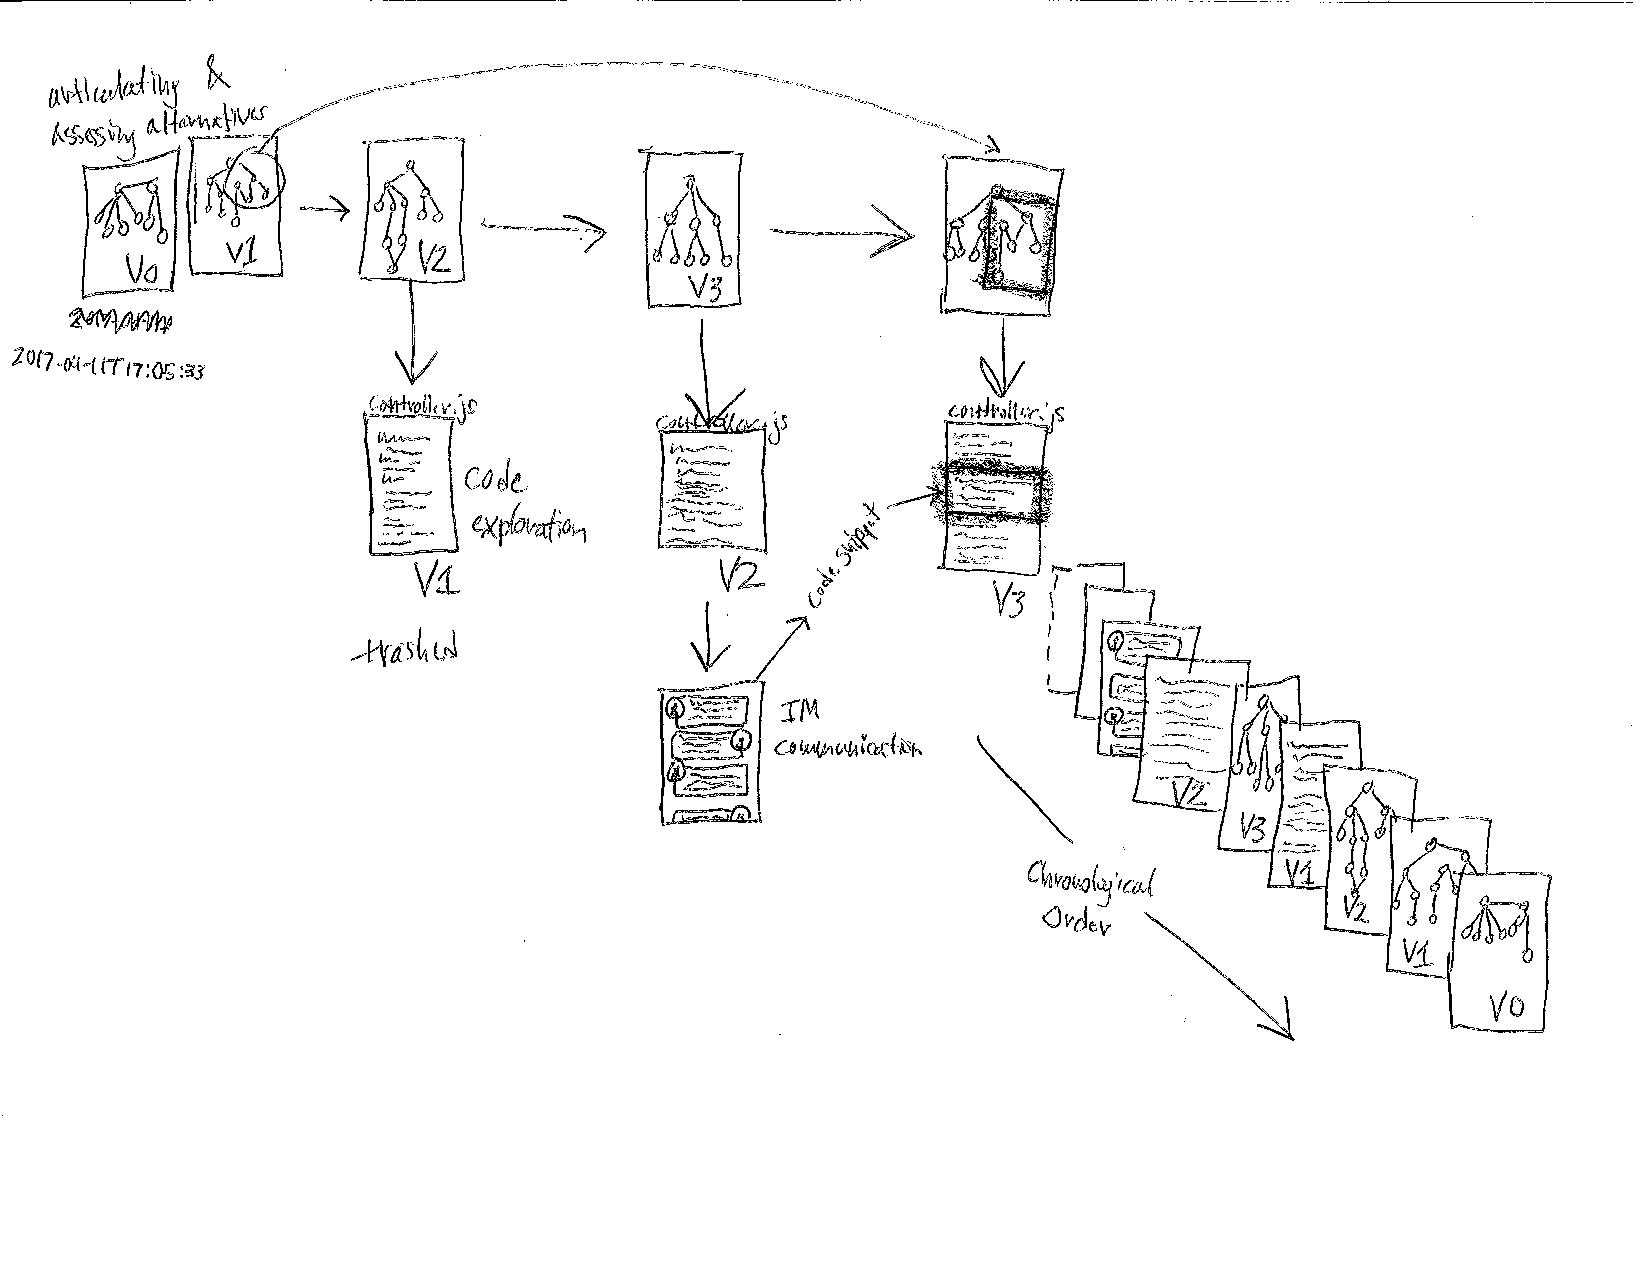
\includegraphics[trim={0 3.5cm 1.0cm 0.6cm},clip,width=\textwidth]{Mockup-7}}
	\vspace*{-1.5\baselineskip}
\end{figure}

Figure~\ref{mockup} displays a high-fidelity mockup of the previous scenario in which Sally is developing a solution to migrate a leaderboard feature to a new shared platform.
She initially creates three sketch cards that contain flow diagrams of three alternative solutions for the problem (cards \texttt{C1-C3}).
Once she has stopped creating new alternatives, she begins to examine the cards already placed on her workspace and decides that the solution on card \texttt{C3} might not be feasible for this particular situation.
To verify this assumption, she opens a code editor card (\texttt{C4}) and begins writing exploratory code in order to validate that this solution does not meet all of the task requirements.
However, during this exploratory development session she realizes that there is another potential solution that could be better than any of her previous alternatives.
She creates another sketch card (\texttt{C5}) to contain that new idea she had, and then a code editor card (\texttt{C6}) to explore the implementation.
After she feels comfortable with this latest solution, she contacts the senior developer on her team via an instant messaging (IM) card (\texttt{c7}) that integrates her Slack conversation into the IDE workspace and shares cards \texttt{C5} and \texttt{C6} to discuss her proposed changes.
The senior developer, Tim, provides some insights into the overall architecture of the game and sends a quick snippet of code that he asks be used to enable a more consistent design across the entire game.
Based on this input, Sally realized that one of her original alternative solutions contains a flow diagram that illustrates Tim's proposed modification exactly.
She creates a copy of card \texttt{C5} and on this card (\texttt{C8}) she also copies the portion of card \texttt{C2} that is desired and combines it with the rest of the flow diagram.
To begin implementing the code, Sally creates another code editor card (\texttt{C9}) and begins coding up the solution she has outlined.
When she reaches the point at which Tim's proposed snippet of code is applicable, she quickly copies and pastes the code from card \texttt{C7} directly into card \texttt{C9}.

This example illustrates the process of \textit{collecting alternative solutions}, 
textit{assessing the feasibility of the alternative solutions}, \textit{examining the applicability of the alternative solutions}, and finally \textit{recombining and consolidating the best aspects into a new solution}.

\section{Conclusions}
Our conclusions are ...


\section{Acknowledgements}
\bold{Add any NSF, OSU, UCI, etc. grants or funding references as needed.}

\bibliography{bibliography}
\bibliographystyle{apacite} 
\end{document}
